\documentclass{article}
\usepackage{amsmath}
\usepackage{graphicx}
\usepackage{epstopdf}
\usepackage{float}
\title{CSL603 - Lab 3\\Multi Layer Perceptron}
\author{Aditya Gupta\\2015CSB1003}
\begin{document}
\maketitle
\section{2-Dimensional 3-Class Classification problem}
\subsection{Goal} Study the changes to the 
\begin{itemize}
\item decision boundary and 
\item the training error
\end{itemize} with respect to parameters such as 
\begin{itemize}
\item number of training iterations,
\item number of hidden layer neurons and
\item finally the learning rate
\end{itemize}
\subsection{MLP Training}
During forward pass, we made $z_h=\sigma(w_h^Tx)$ and $y'_k=\sigma(v_k^Tz)$ (The weights and points had different orientation to what discussed in class, therefore an appropriate formula equivalent to these was used.)
During backpropagation, for a particular point we used $$\Delta v_{hk}=\underbrace{\eta(y'_k-y_k)y'_k(1-y'_k)}_{\text{Common for a particular } k}z_h$$ and $$\Delta w_{jh}=\underbrace{\eta\left(\sum_k(y'_k-y_k)y'_k(1-y'_k)v_{hk}\right)z_h(1-z_h)}_{\text{Common for a particular }h}x_j$$ (Various values were calculated only once which were common for a particular $k$ for $\Delta v_{hk}$ and these were further used in case of $\Delta w_{jh}$, moreover the common values in case of $\Delta w_{jh}$ for a particular $h$ were also calculated only once.)
\subsection{Training Error}
The training error for all the points was summed up to get $E=\frac 12\Sigma||y'_i-y_i||^2$ where the subscript denotes $i$-th point, rather than the $i$-th dimension for a particular point.
\subsection{MLP Testing}
The similar formulas as for MLP training were used but here, instead we had multiple points, so an appropriate form was used (The bias term was introduced differently which in this case would be a column vector, rest was same).
\subsection{Observations}
Parameters: $\eta=0.0001,$ \verb|nEpochs| $=1000$. The value of $H$ was varied as $2,4,8,16,32$ and $64$. The following graphs for the error versus number of epochs the were obtained:
\begin{figure}[H]
\makebox[\textwidth][c]{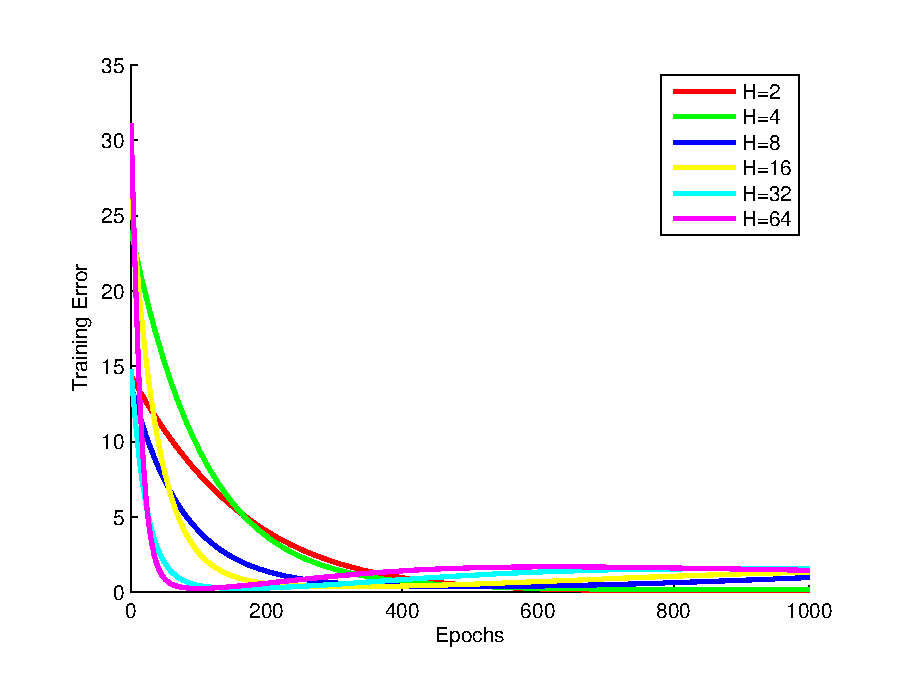
\includegraphics[scale=0.6]{figure1.eps}}
 \caption{Change in Training Error as a function of total number of epochs varied across the number of nodes in the hidden layer. Here $\eta=0.0001$ (learning rate)}
 \label{fig:1}
 \end{figure}
 The value of H was now varied as $2,4$ and $64$ and the following decision boundaries were obatined:
 \begin{figure}[H]
\makebox[\textwidth][c]{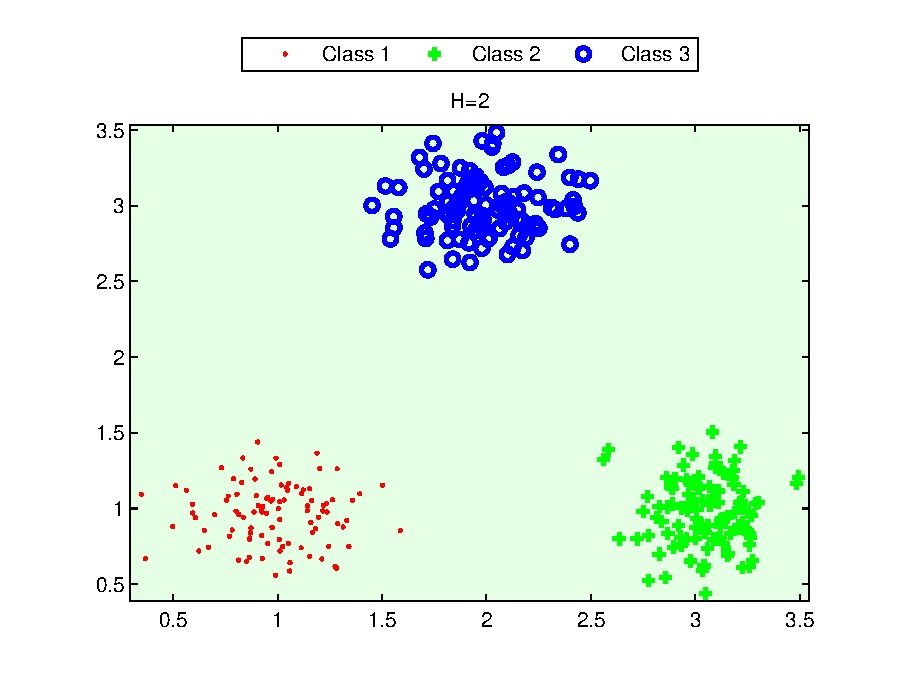
\includegraphics[scale=1]{h2f2.eps}}
 \caption{Decision Boundary for $H=2$}
 \label{fig:2}
 \end{figure}
  \begin{figure}[H]
\makebox[\textwidth][c]{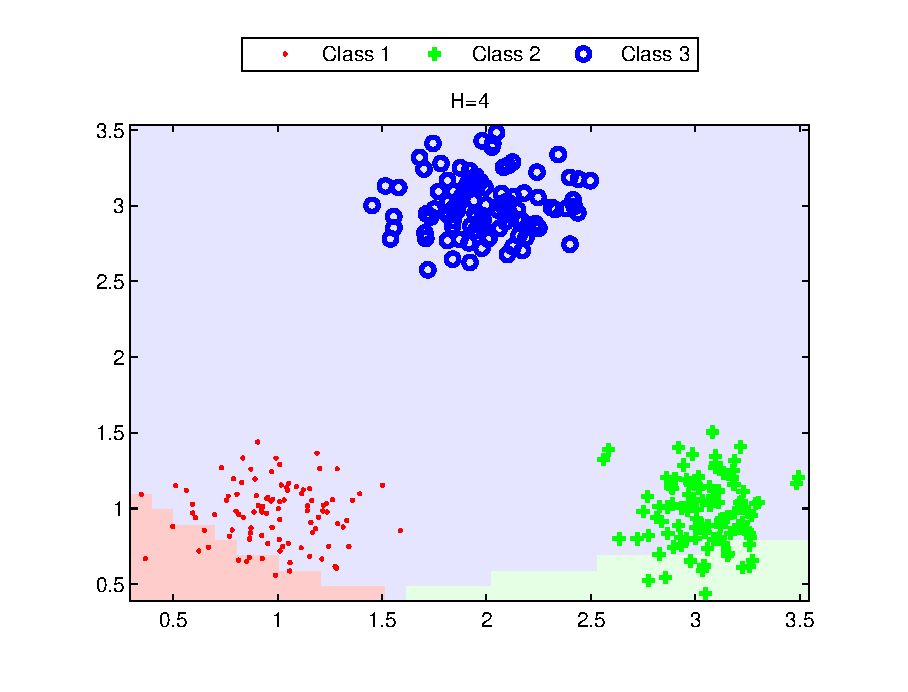
\includegraphics[scale=1]{h4f2.eps}}
 \caption{Decision Boundary for $H=4$}
 \label{fig:3}
 \end{figure}
  \begin{figure}[H]
\makebox[\textwidth][c]{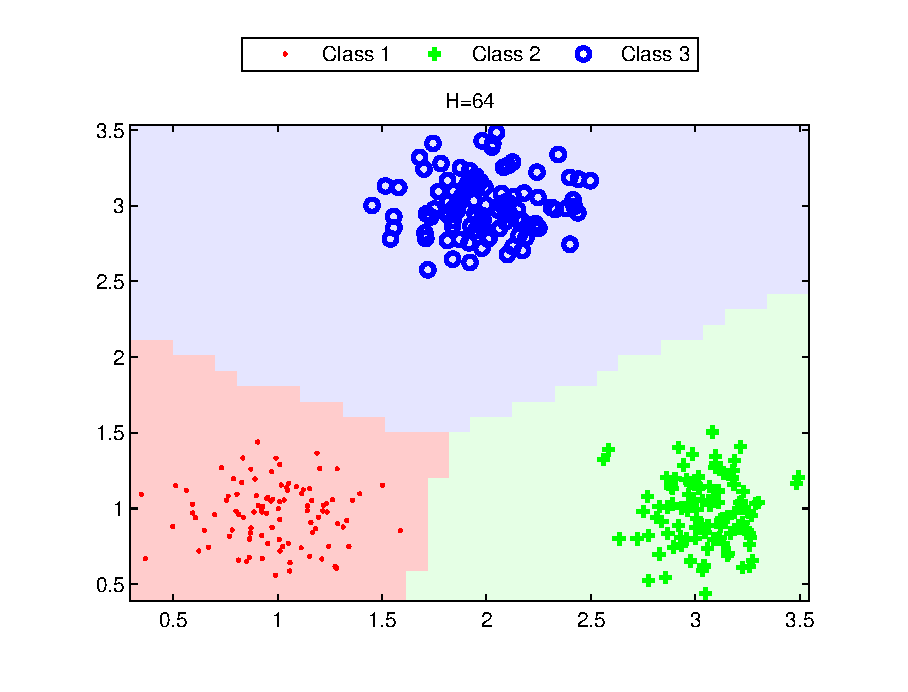
\includegraphics[scale=1]{h64f2.eps}}
 \caption{Decision Boundary for $H=64$}
 \label{fig:4}
 \end{figure}
\subsection{Discussion and Conclusions}
\end{document}